\section{INTRODUCTION}

The \textit{rnucs} tally has been implemented in MCNP6.2. In order
to assess the correct implemetation of the tally, a quantitative
comparison to the tally implemented in MCNP6.1 has been performed.

\section{COMPARISON OF RNUCS IN MCNP6.1 AND MCNP6.2}

\subsection{Geometry}
A simple geometry was selected for this comparison. 
The geometry consist of a single mercury volume as can be seen in Figure \ref{fig:merbox.png}.
A Gaussian distribution centered around 1GeV proton source was used. 
The source is located in the xy plane at z = -256.71 cm, where the x position is
dependent on the y position. 


\begin{figure}[h!]
        \centering
        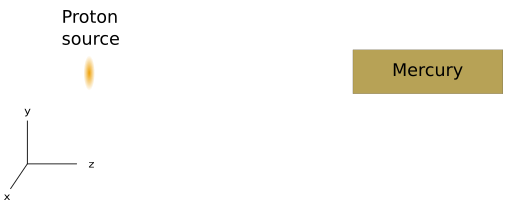
\includegraphics[scale=0.7]{figs/mercury.png}
        \caption[VPI]{Planar view of the testing geometry}
        \label{fig:merbox.png}
\end{figure}


\subsection{MCNP Transport}
A transport calculation was performed with MCNP6.1 and MCNP6.2 and 1E8 histories.
The \textit{rnucs} tally was used in both calculaitons to obtain
the isotope production and destruction in the mercury volume
Figures \ref{fig:prod} and \ref{fig:dest}  show the isotope production
and isotope destruction collected in the mercury volume. These figures also
show the relative difference between the results collected in MCNP6.1
and MCNP6.2. 
The relative difference is given by the following equation:
\begin{equation}
	\frac{MCNP6.2 - MCNP6.1}{MCNP6.1}.
\end{equation}


\begin{figure}[h!]
        \centering
        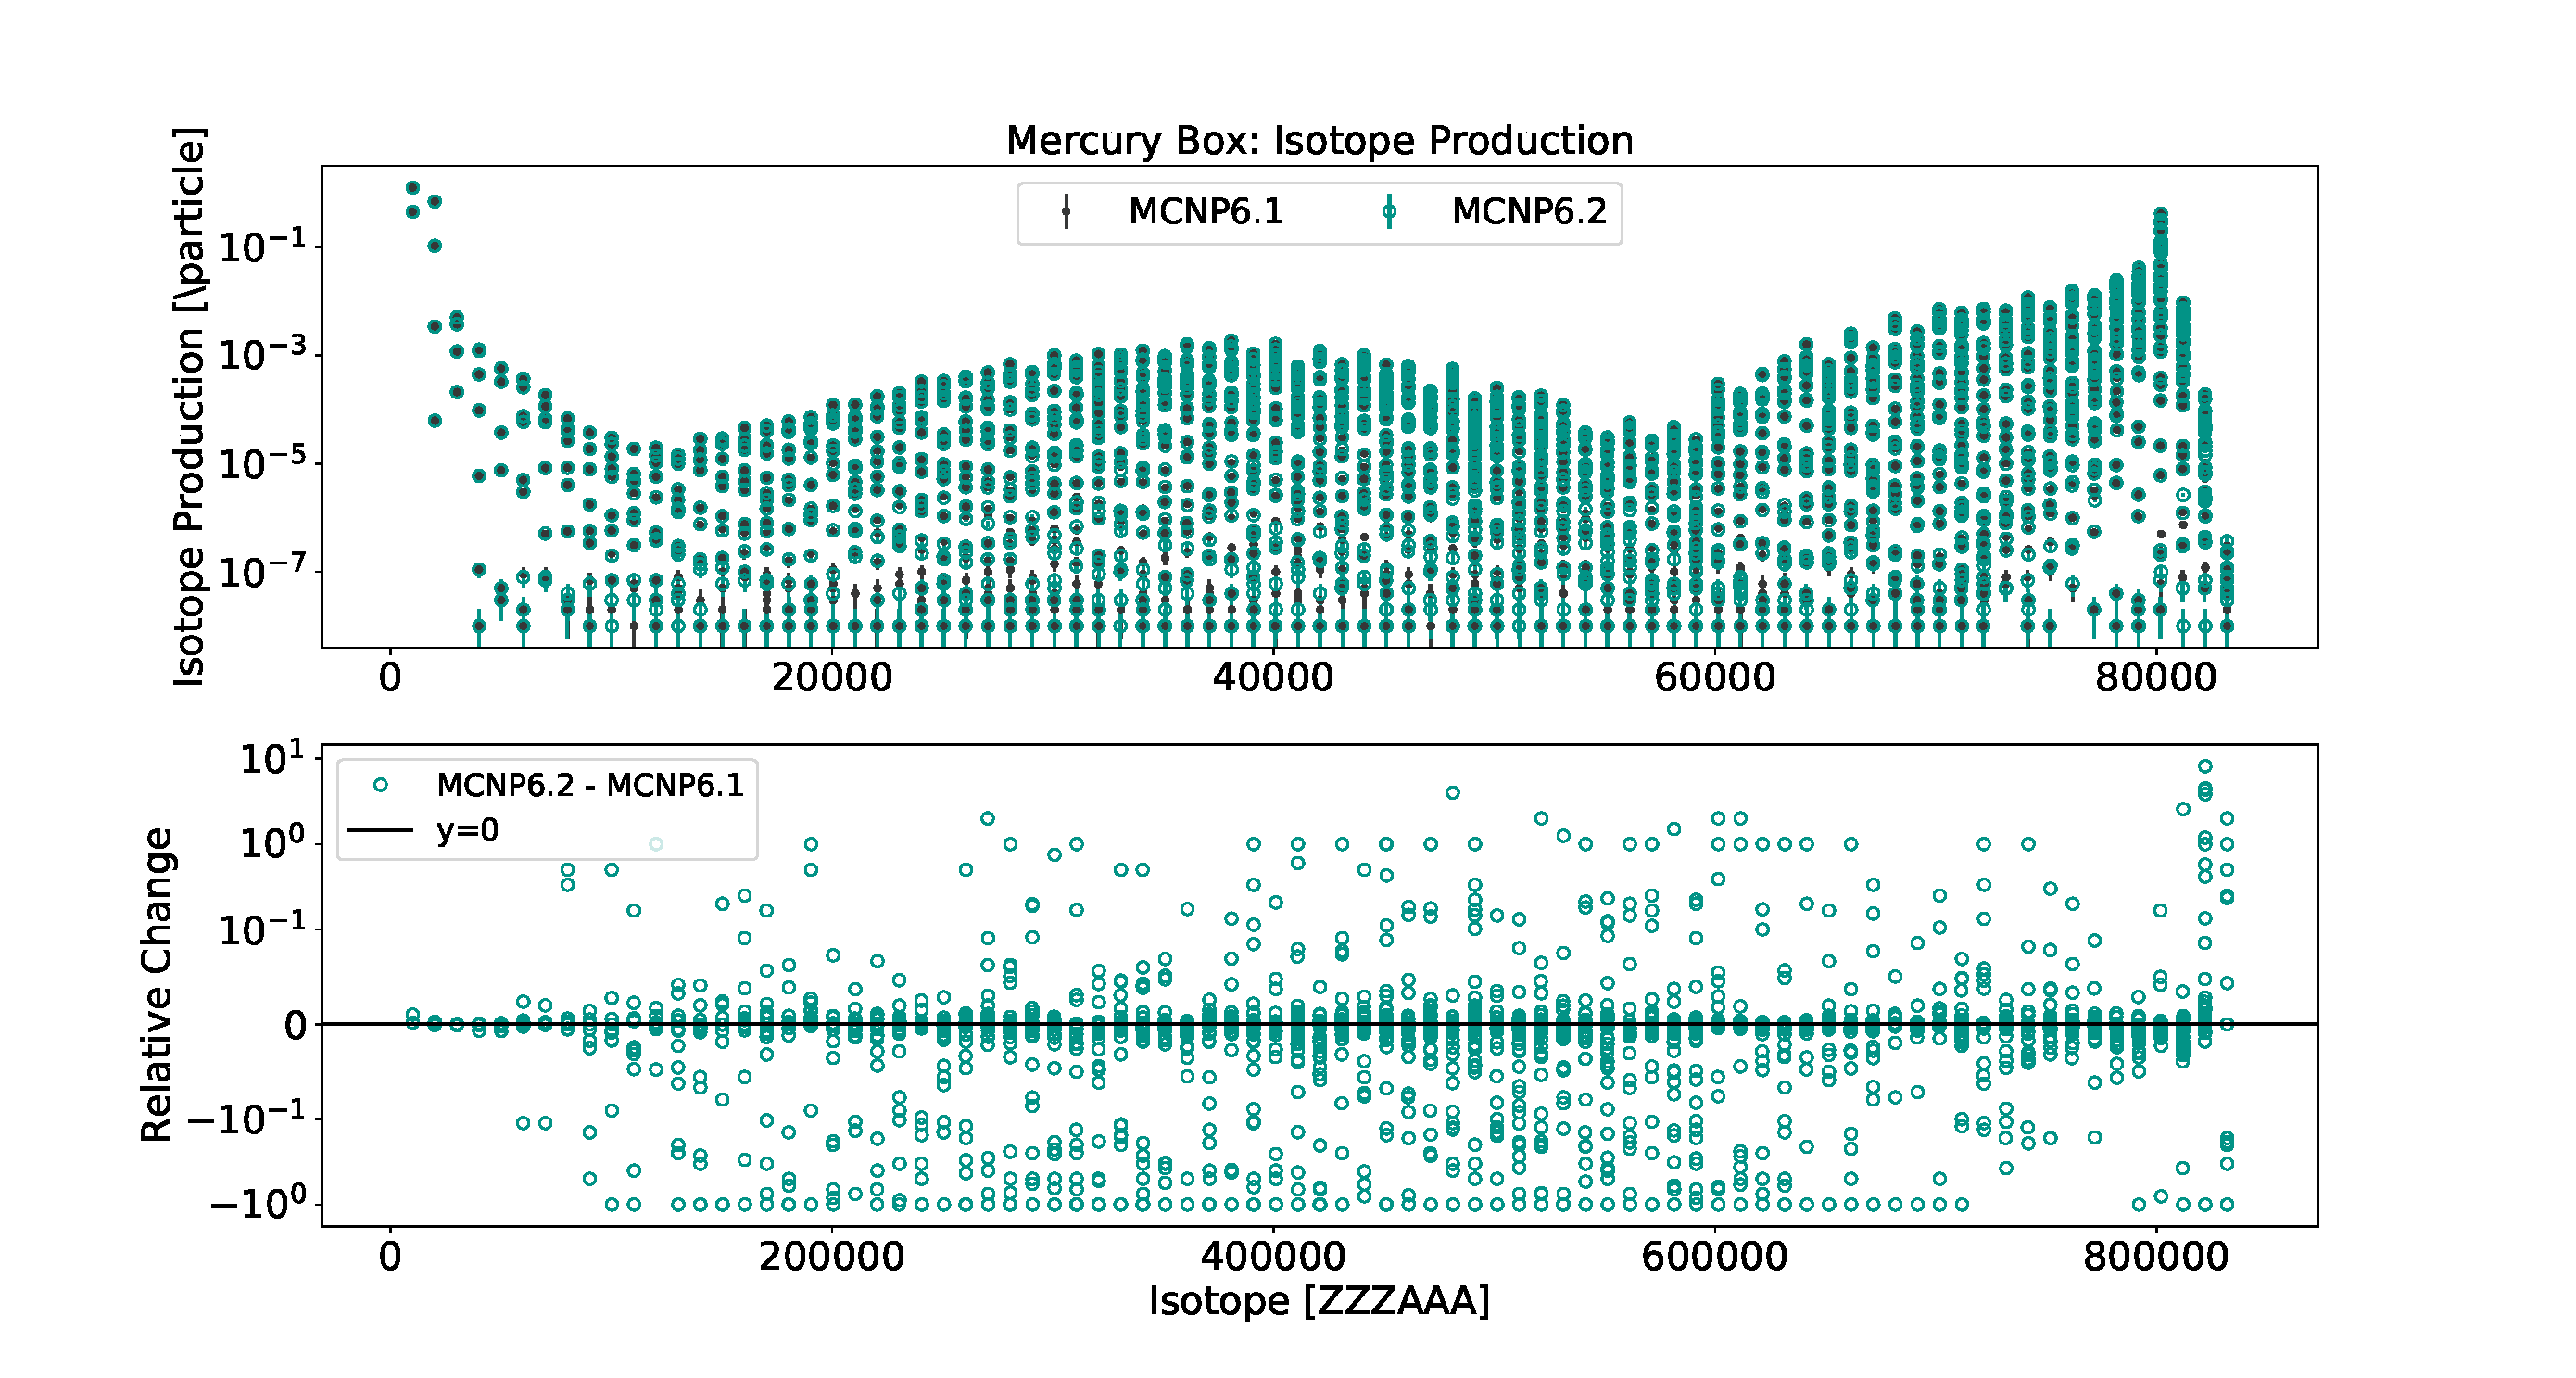
\includegraphics[scale=0.4]{figs/prod_merbox_62_61.pdf}
	\caption{Isotope Production in the Mercury volume}
        \label{fig:prod}
\end{figure}

\begin{figure}[h!]
        \centering
        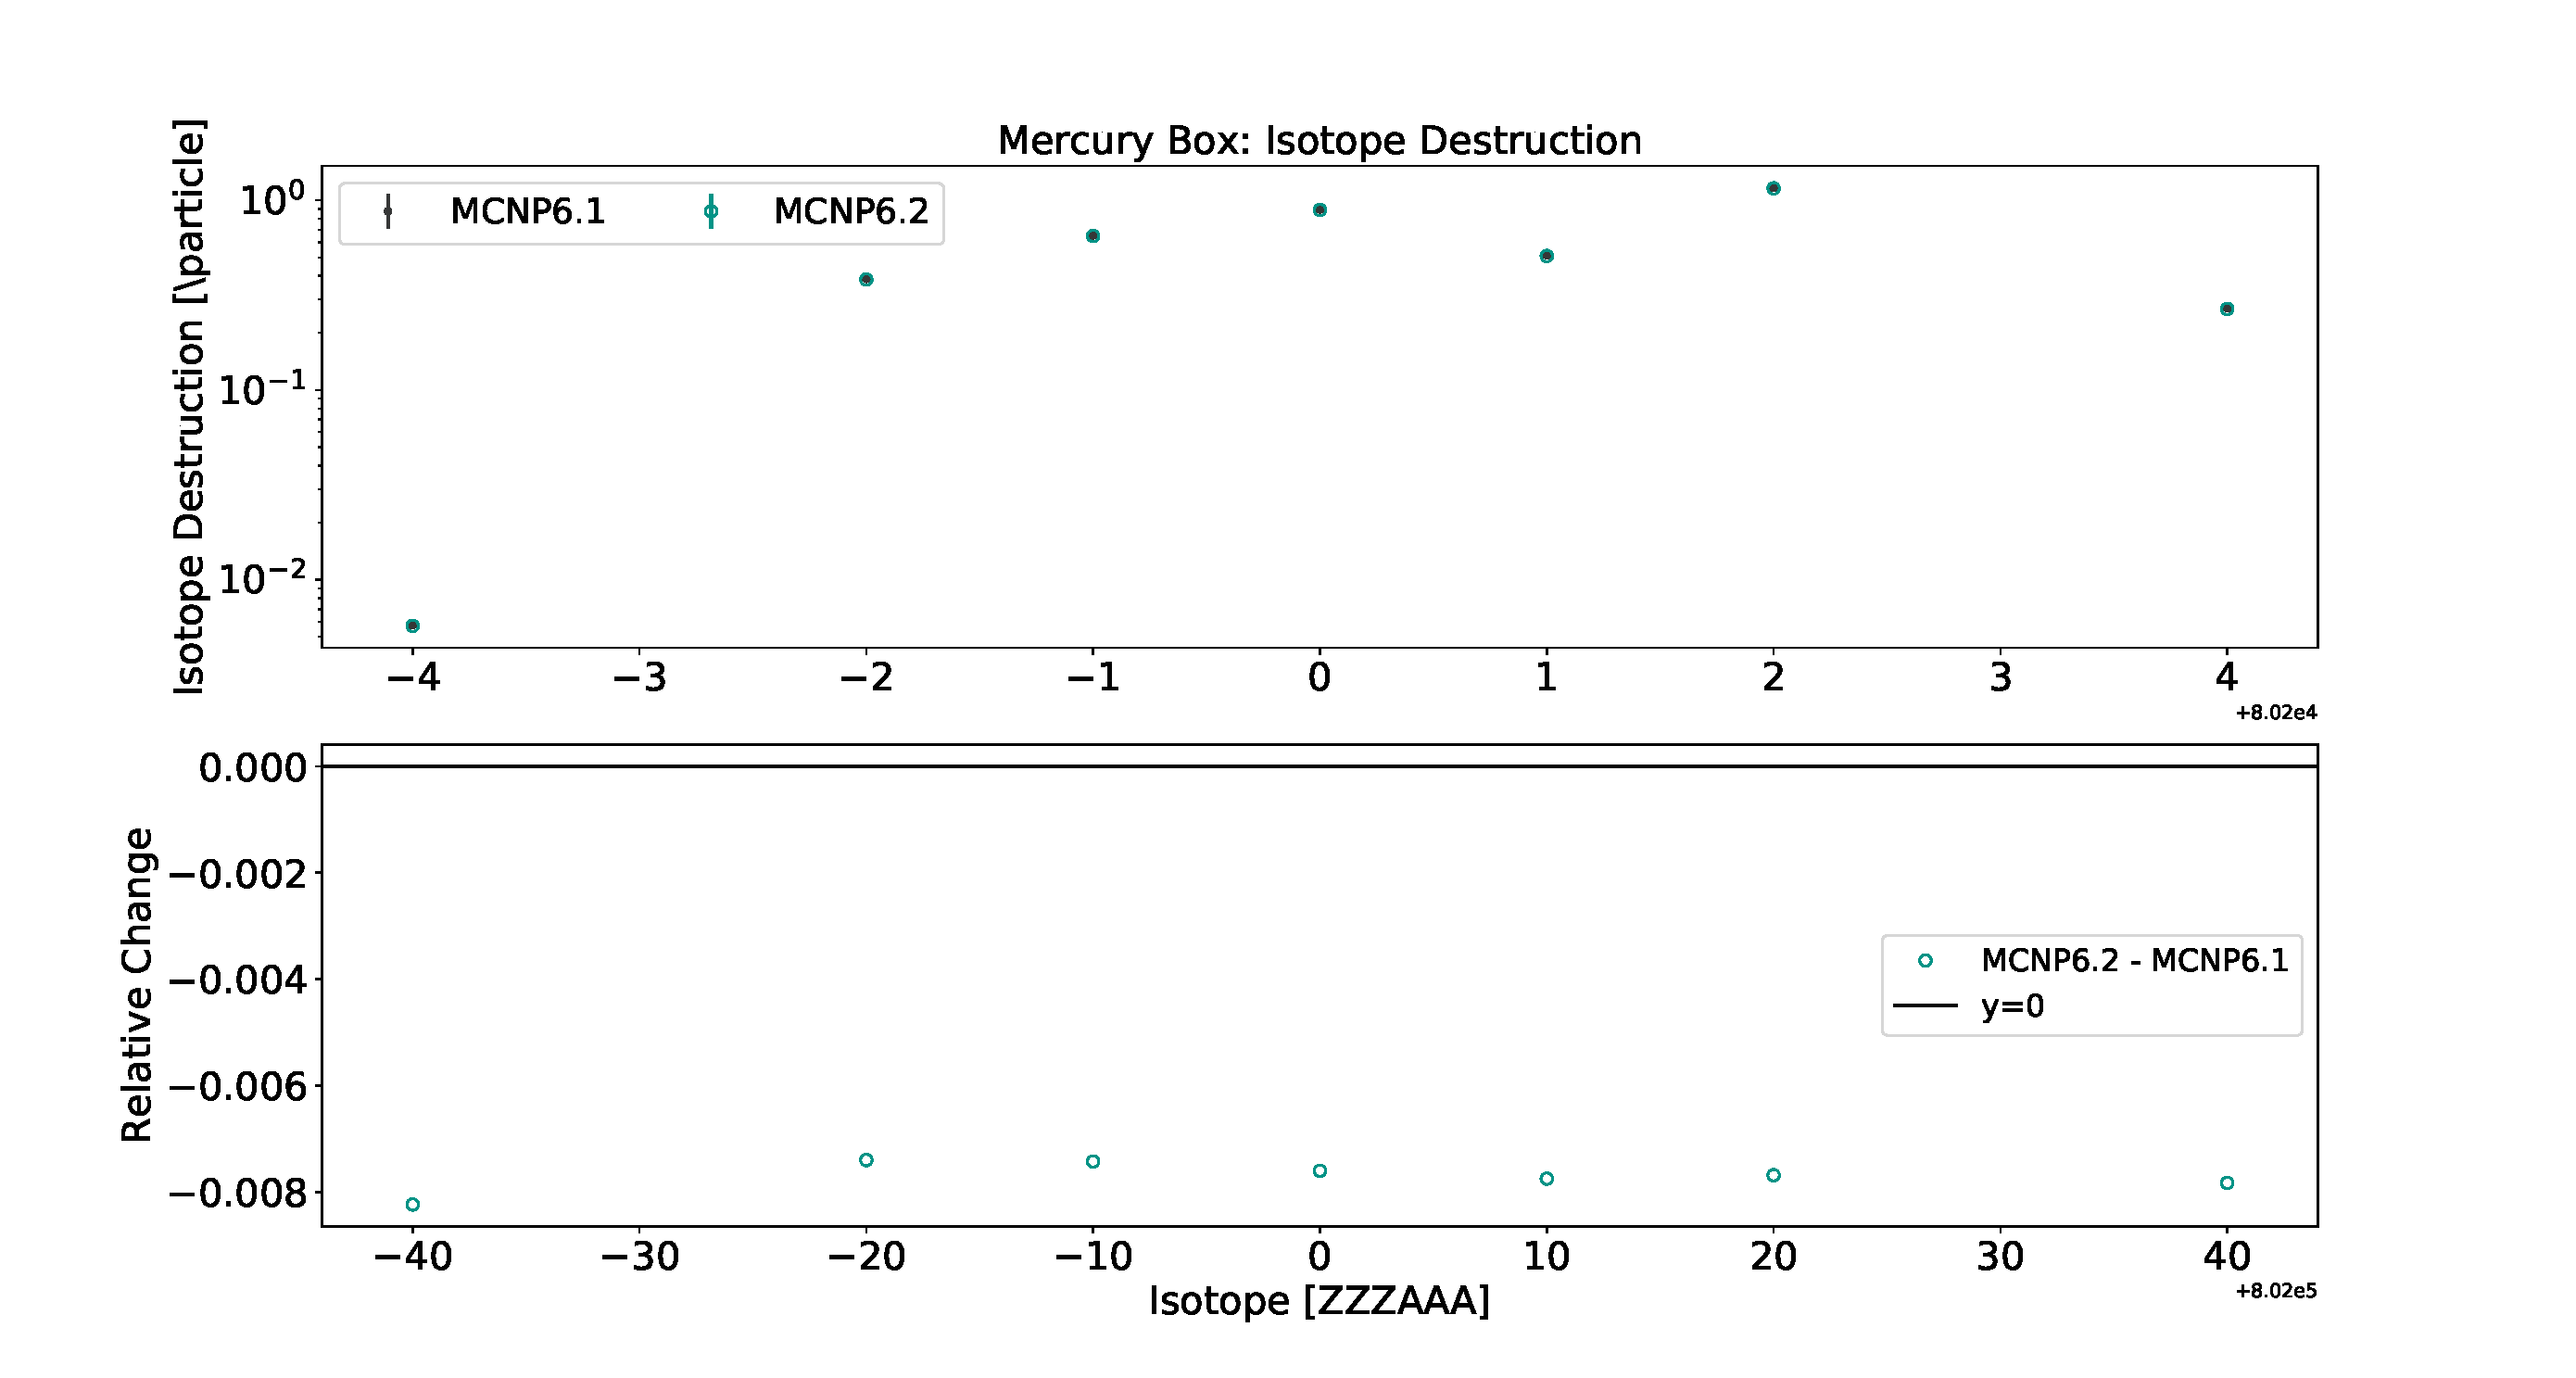
\includegraphics[scale=0.4]{figs/dest_merbox_62_61.pdf}
	\caption{Isotope Destruction in the Mercury volume}
        \label{fig:dest}
\end{figure}

Figure \ref{fig:prod} shows that for many isotopes the isotope 
production obtained in MCNP6.2 is significantly different than the
isotope production obatined in MNCP6.1. 
To better understand the importance of
the difference, a graph representing the relative difference versus the
isotope production data in MCNP6.1 is shown in Figure \ref{fig:reldiff}. This 
figure tells us that most of the isotopes with high relative difference
have a low isotope production.

\begin{figure}[h!]
        \centering
        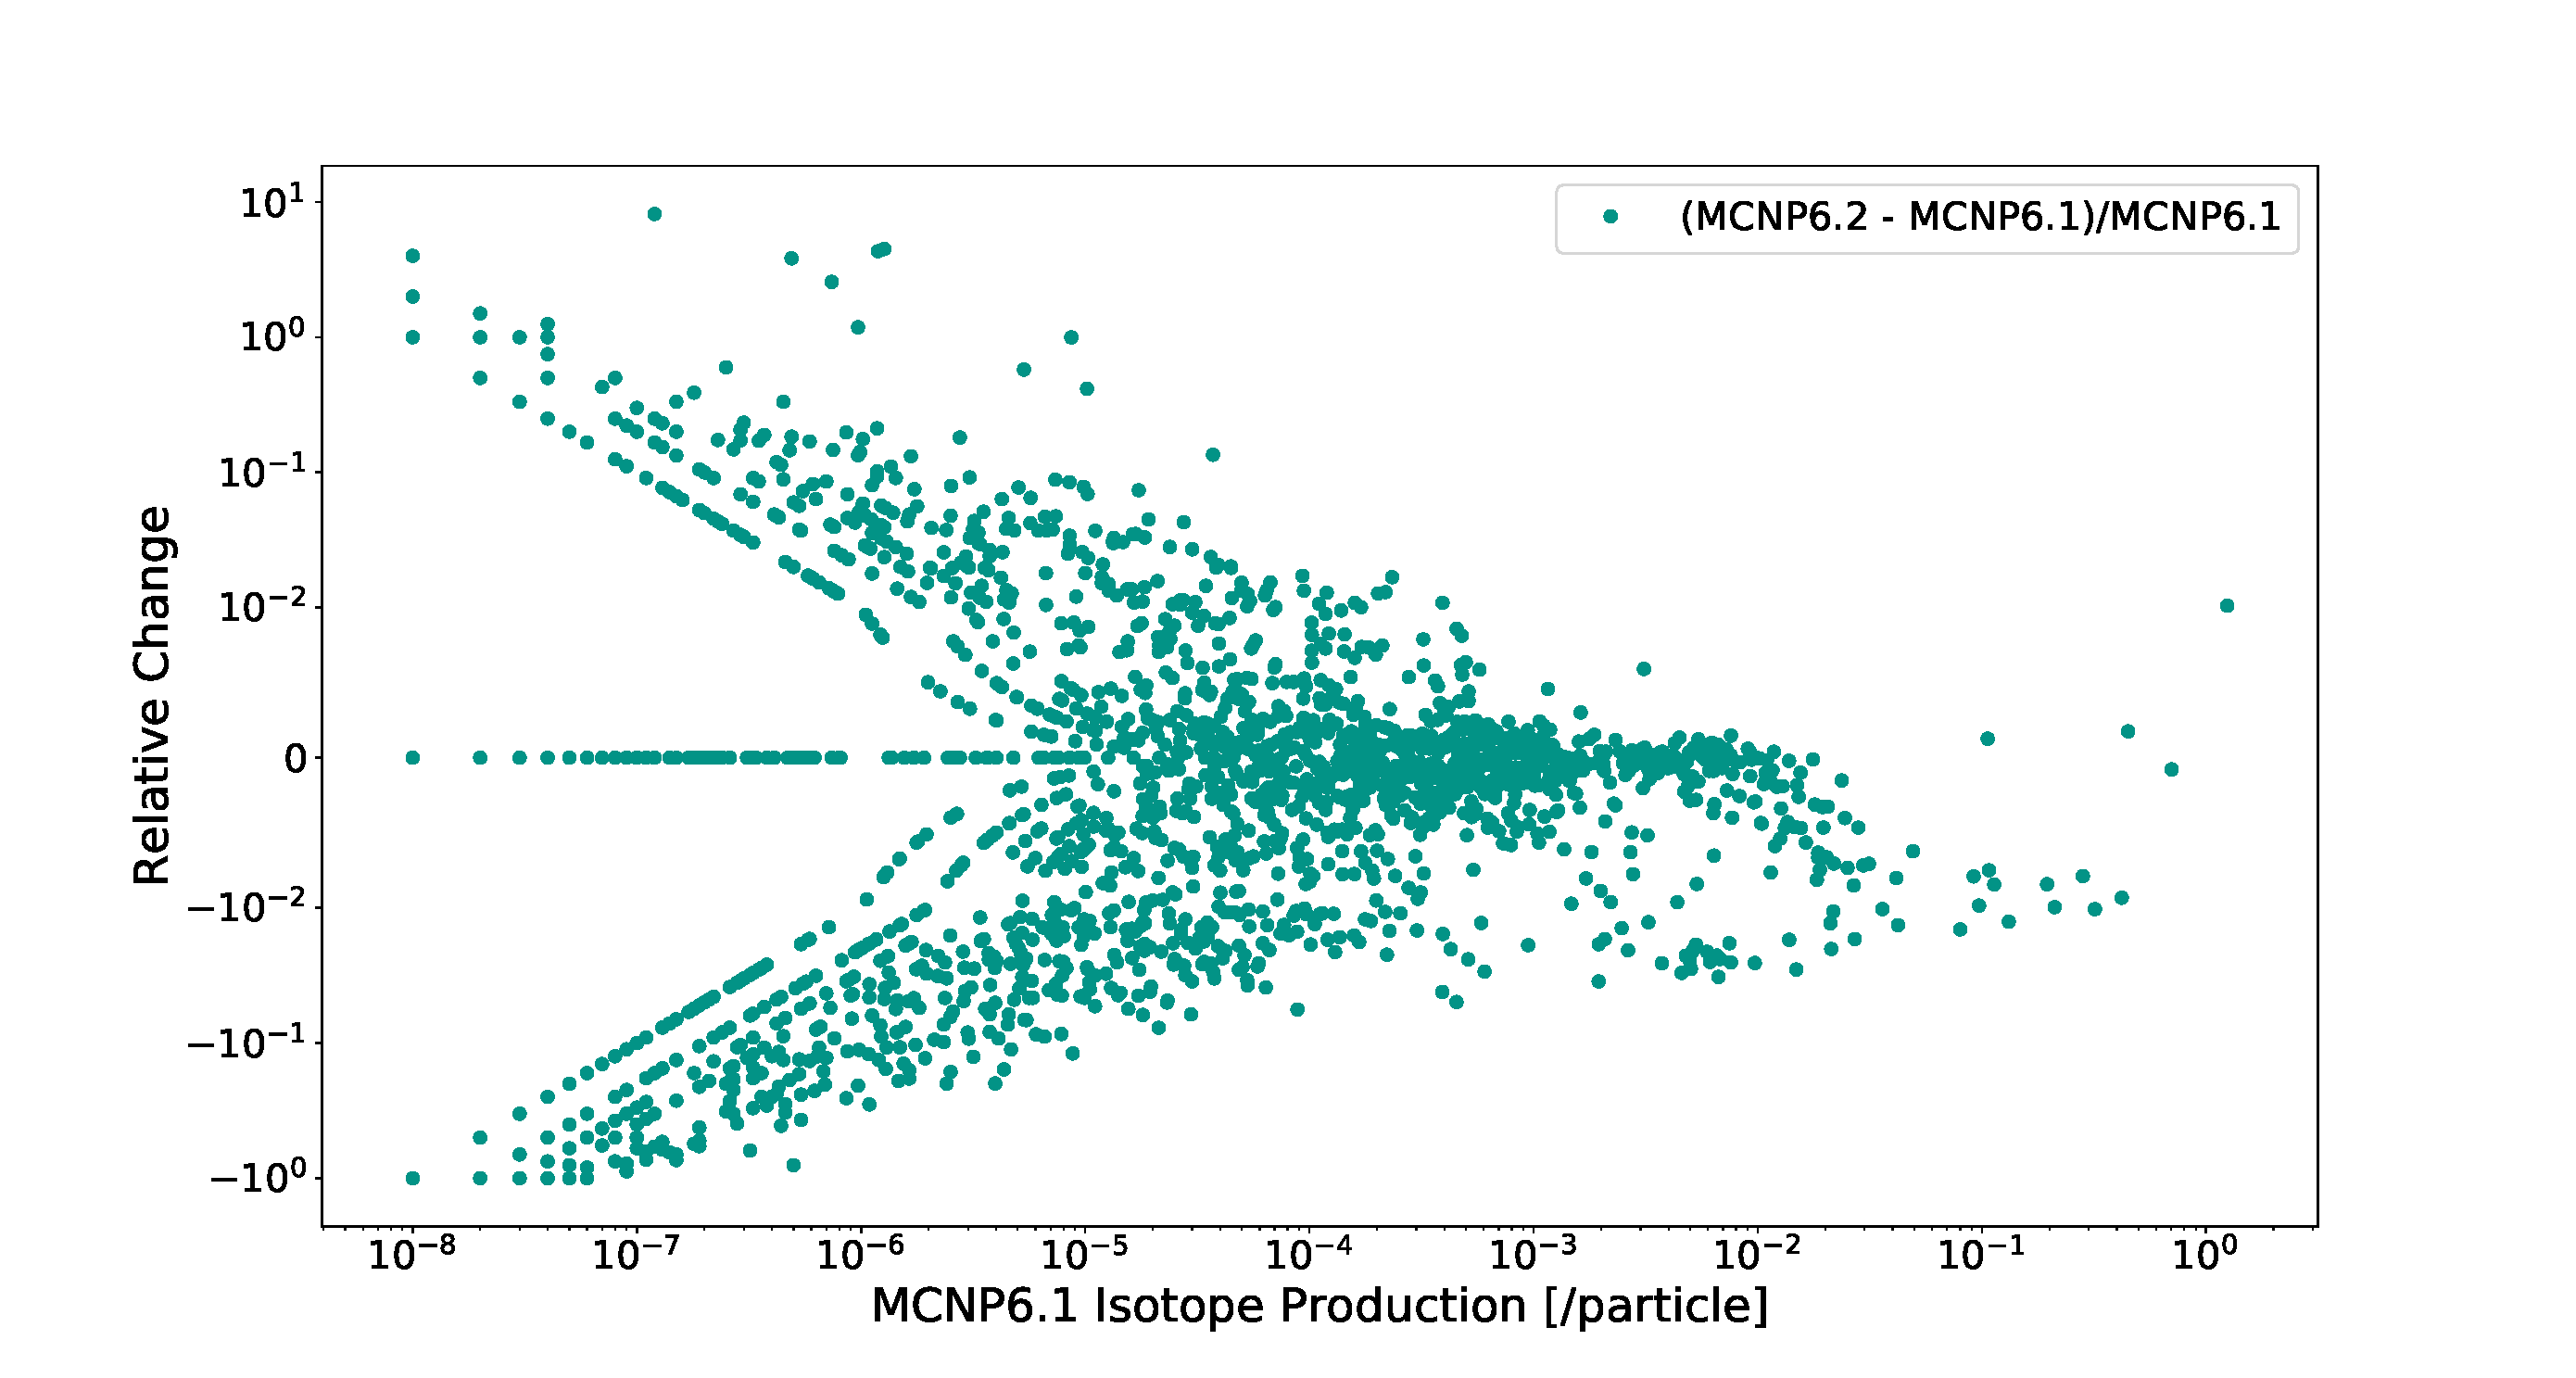
\includegraphics[scale=0.4]{figs/reldiff_merbox_62_61.pdf}
	\caption{Relative Difference vs. Isotope Production}
        \label{fig:reldiff}
\end{figure}

Another metric used in this work to compare the results is the Z-Score quatity.
A Z-score
is a quantity that tells us how many standard deviations a value is from a
population
mean. In this comparison, two sample means are compare and the following
equation was used. 
\begin{equation}\label{eq:ztest}
        z = \frac{(\bar{x}_{1} - \bar{x_{2}}) - (\mu_{1} - \mu_{2}) }
            {\sqrt{\frac{\sigma_{1}^{2}}{n_{1}} + \frac{\sigma_{2}^{2}}{n_{2}} }}
\end{equation}
where
\begin{equation}
\begin{split}
        \bar{x} &= \text{Sample mean} \\
        \mu     &= \text{Population mean} \\
        \sigma  &= \text{Population standard deviation} \\
        n       &= \text{Sample size}
\end{split}
\end{equation}

Figure \ref{fig:pdf} shows the PDF of Z-scores when comparing 
the isotope production of MNCP6.1 and MCNP6.2. 
\begin{figure}[h!]
        \centering
        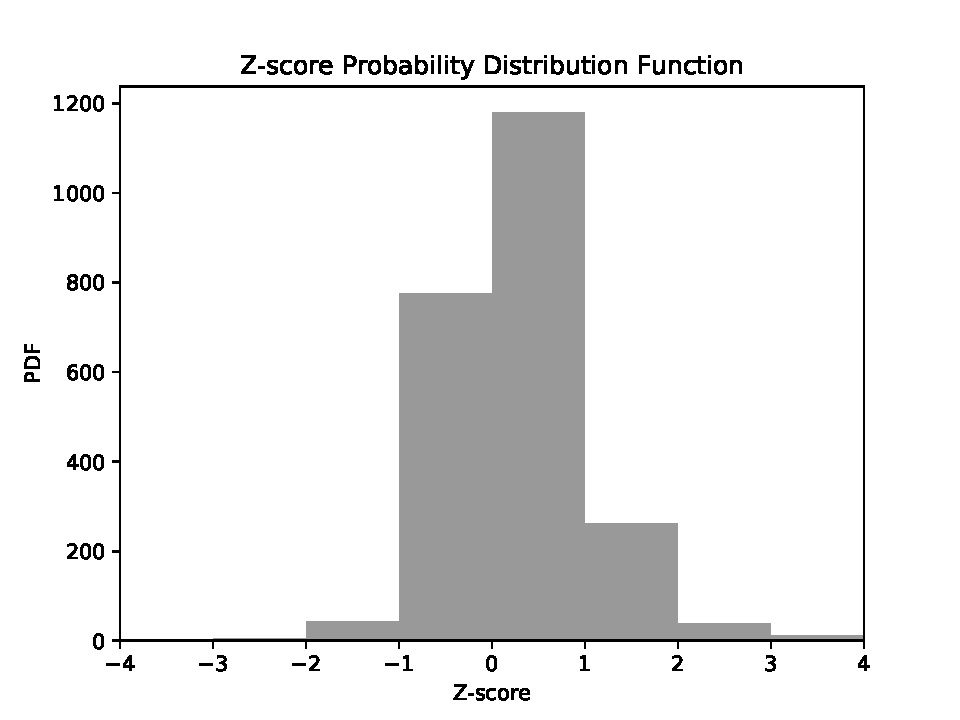
\includegraphics[scale=0.4]{figs/PDF.pdf}
        \caption{Z-scores PDF }
        \label{fig:reldiff}
\end{figure}


\begin{center}
\begin{tabular}{ |c|c|c|c|}
 \hline
 voxels with: & z $\leq 1 \sigma$ & z $\leq 2 \sigma$ & z $\leq 3 \sigma$ \\
 \hline \hline
              & 85.03 \%          & 94.29 \%          & 95.96 \%           \\
 \hline
\end{tabular}
\end{center}

